% Results figures, rendered from the persisted artifacts:
% bootstrap_ci.json (suite means and 95% CIs), stability_run1_vs_run2.json (run pairs).
% Layout discipline: the top panel shows point estimates + intervals only
% (no filled bars under the whiskers), the bottom panel's legend lives
% below the axis (never over the bars), and both panels share the same
% value range so the stacked scales read as one.
\begin{figure}[t]
\centering
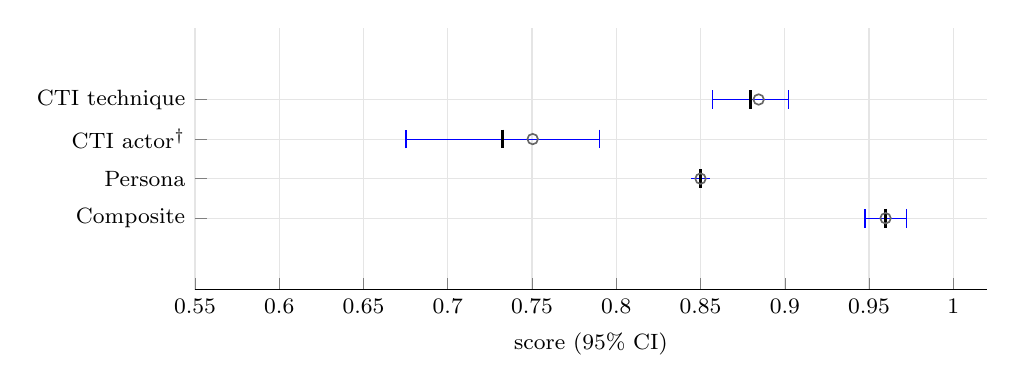
\begin{tikzpicture}
\begin{axis}[
  name=ax1,
  width=0.96\linewidth,
  height=4.9cm,
  xmin=0.55, xmax=1.02,
  y axis line style={draw=none},
  axis x line*=bottom,
  axis y line*=left,
  ytick=data,
  yticklabels={Composite,Persona,CTI actor$^{\dagger}$,CTI technique},
  y dir=reverse,
  xlabel={score (95\% CI)},
  xlabel style={font=\footnotesize},
  tick label style={font=\footnotesize},
  enlarge y limits=0.6,
  grid=major,
  grid style={black!10},
  clip=false
]
% point estimates and bootstrap 95% CIs from bootstrap_ci.json;
% only marks + intervals: no bars beneath the whiskers
\addplot+[only marks, mark=|, mark size=3.4, mark options={thick,black},
  error bars/.cd, x dir=both, x explicit] coordinates {
  (0.9598,3) +- (0.0122,0.0122)
  (0.8500,2) +- (0.0000,0.0000)
  (0.7325,1) +- (0.0573,0.0558)
  (0.8796,0) +- (0.0224,0.0204)
};
% run-2 overlay: open markers (point estimates from stability_run1_vs_run2.json;
% per-suite CIs were not computed for run 2, so none are drawn)
\addplot+[only marks, mark=o, mark size=1.9, mark options={semithick,black!60}] coordinates {
  (0.9598,3)
  (0.8500,2)
  (0.7504,1)
  (0.8845,0)
};
\end{axis}
\end{tikzpicture}

\vspace{2mm}

\begin{tikzpicture}
\begin{axis}[
  name=ax2,
  width=0.96\linewidth,
  height=4.9cm,
  ybar=1.5pt,
  bar width=9pt,
  ymin=0.55, ymax=1.0,
  symbolic x coords={CTI technique,CTI actor,Persona,Composite},
  xtick=data,
  ylabel={mean score},
  ylabel style={font=\footnotesize},
  tick label style={font=\footnotesize},
  ymajorgrids,
  grid style={black!10},
  enlarge x limits=0.25,
  legend style={font=\scriptsize, at={(0.5,-0.16)}, anchor=north, legend columns=2, draw=none, fill=none},
  legend cell align={left},
]
% run 1 vs run 2 from stability_run1_vs_run2.json
\addplot+[black!35, fill=black!35] coordinates {
  (CTI technique,0.9598) (CTI actor,0.8500) (Persona,0.7325) (Composite,0.8796)
};
\addplot+[black!70, fill=black!70, pattern=north east lines] coordinates {
  (CTI technique,0.9598) (CTI actor,0.8500) (Persona,0.7504) (Composite,0.8845)
};
\legend{run 1, run 2}
\end{axis}
\end{tikzpicture}
\caption{Live-campaign results from the persisted artifacts. \emph{Top:}
suite means with bootstrap 95\% confidence intervals; open markers mark
the independent second run's point estimates, and the actor interval is
degenerate ($^{\dagger}$) because the actor rubric assigns the same
score to every row, so uncertainty is carried by the Wilson pass-rate
interval instead (Table~\ref{tab:live}). \emph{Bottom:} two independent
218-query campaigns; the deterministic CTI strata replicate exactly and
only the LLM-judged persona stratum moves, by $+0.018$.}
\label{fig:results}
\end{figure}
